% Les fonctions se construisent les unes sur les autres
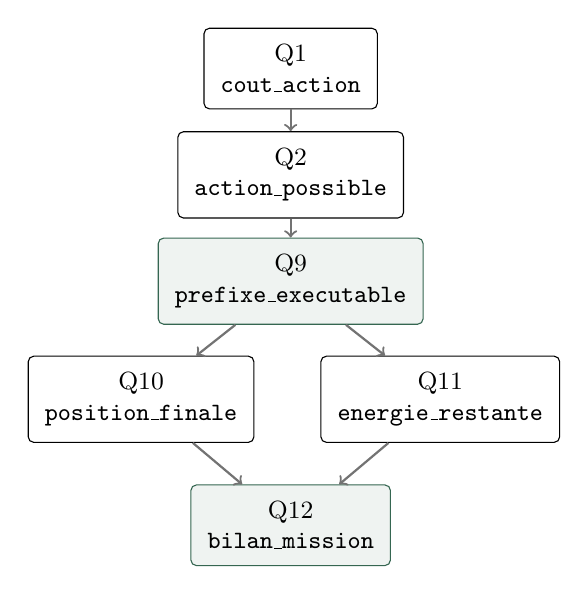
\begin{tikzpicture}[font=\small,
bloc/.style={draw,rounded corners=2pt,align=center,inner sep=6pt},
lien/.style={->,thick,draw=black!55}]
\definecolor{vert}{RGB}{53,102,81}
\node[bloc] (cout) at (0,0) {Q1\\\texttt{cout\_action}};
\node[bloc] (possible) at (0,-1.35) {Q2\\\texttt{action\_possible}};
\node[bloc,draw=vert,fill=vert!8] (prefixe) at (0,-2.7) {Q9\\\texttt{prefixe\_executable}};
\node[bloc] (position) at (-1.9,-4.2) {Q10\\\texttt{position\_finale}};
\node[bloc] (energie) at (1.9,-4.2) {Q11\\\texttt{energie\_restante}};
\node[bloc,draw=vert,fill=vert!8] (bilan) at (0,-5.8) {Q12\\\texttt{bilan\_mission}};
\draw[lien] (cout) -- (possible);
\draw[lien] (possible) -- (prefixe);
\draw[lien] (prefixe) -- (position);
\draw[lien] (prefixe) -- (energie);
\draw[lien] (position) -- (bilan);
\draw[lien] (energie) -- (bilan);
\end{tikzpicture}
